%!TEX root = ../thesis.tex
%*******************************************************************************
%****************************** Third Chapter **********************************
%*******************************************************************************
\graphicspath{{Chapter3/Figs/Vector/}{Chapter3/Figs/}}

%%%%%%%%%%%%%%%%%%%%%%%%%%%%%%%%%%%%%%%%%%%%%%%%%%%%%%%%%%%%%%%%%%%%%%%%%%%%%%%%
% System Architecture
%%%%%%%%%%%%%%%%%%%%%%%%%%%%%%%%%%%%%%%%%%%%%%%%%%%%%%%%%%%%%%%%%%%%%%%%%%%%%%%%
% - What is most fitting solution to integrate TPS and UI into the
%   existing architecture?
%
\chapter{System Architecture}
\section{Introduction}
In order to succesfully integrate a new system component in an existing system architecture, flows of information must be aligned with adjacent system components, so that data dependencies of the new component are satisfied, and expected functionalities can be provided in return. This chapter explains which important aspects dictate the systems architecture to implement TPS.

%%%%%%%%%%%%%%%%%%%%%%%%%%%%%%%%%%%%%%%%%%%%%%%%%%%%%%%%%%%%%%%%%%%%%%%%%%%%%%%%
% Architectural Patterns
%%%%%%%%%%%%%%%%%%%%%%%%%%%%%%%%%%%%%%%%%%%%%%%%%%%%%%%%%%%%%%%%%%%%%%%%%%%%%%%%
% - Which architectural patterns fit in with the exising architecture?
%
\section{Architectural Patterns}
The current system architecture consists of three API's and nine services that connect to four databases, as can be seen in figure \ref{fig:Architecture}. They provide functionalities to portals and mobile apps. The user interface, business logic, and data storage are separated, following the three-tier or multi-tier architecture \cite{IBM-3-tier}. The bigger and smaller shapes in the figure represent large API's and services respectively. The orange colored services are used internally, the green ones can be used by other companies. The smaller services adhere to the pattern that is called service-oriented architecture (SOA), where application components provide services over a network typically.

Developers have carefully constructed the components that comprise the system architecture, designing their relations, taking evolution of the architecture into account. This design is to be respected and utilized in a way that does not hinder the planned evolution.

% ! indicates that some restrictions should be ignored
% h indicates that the float is allowed to be placed inline
% t indicates that the float is allowed to go into a top area
% b indicates that the float is allowed to go into a bottom area
% p indicates the the float is allowed to go on a float page or column area

\begin{figure}[!htb]
	\centering
	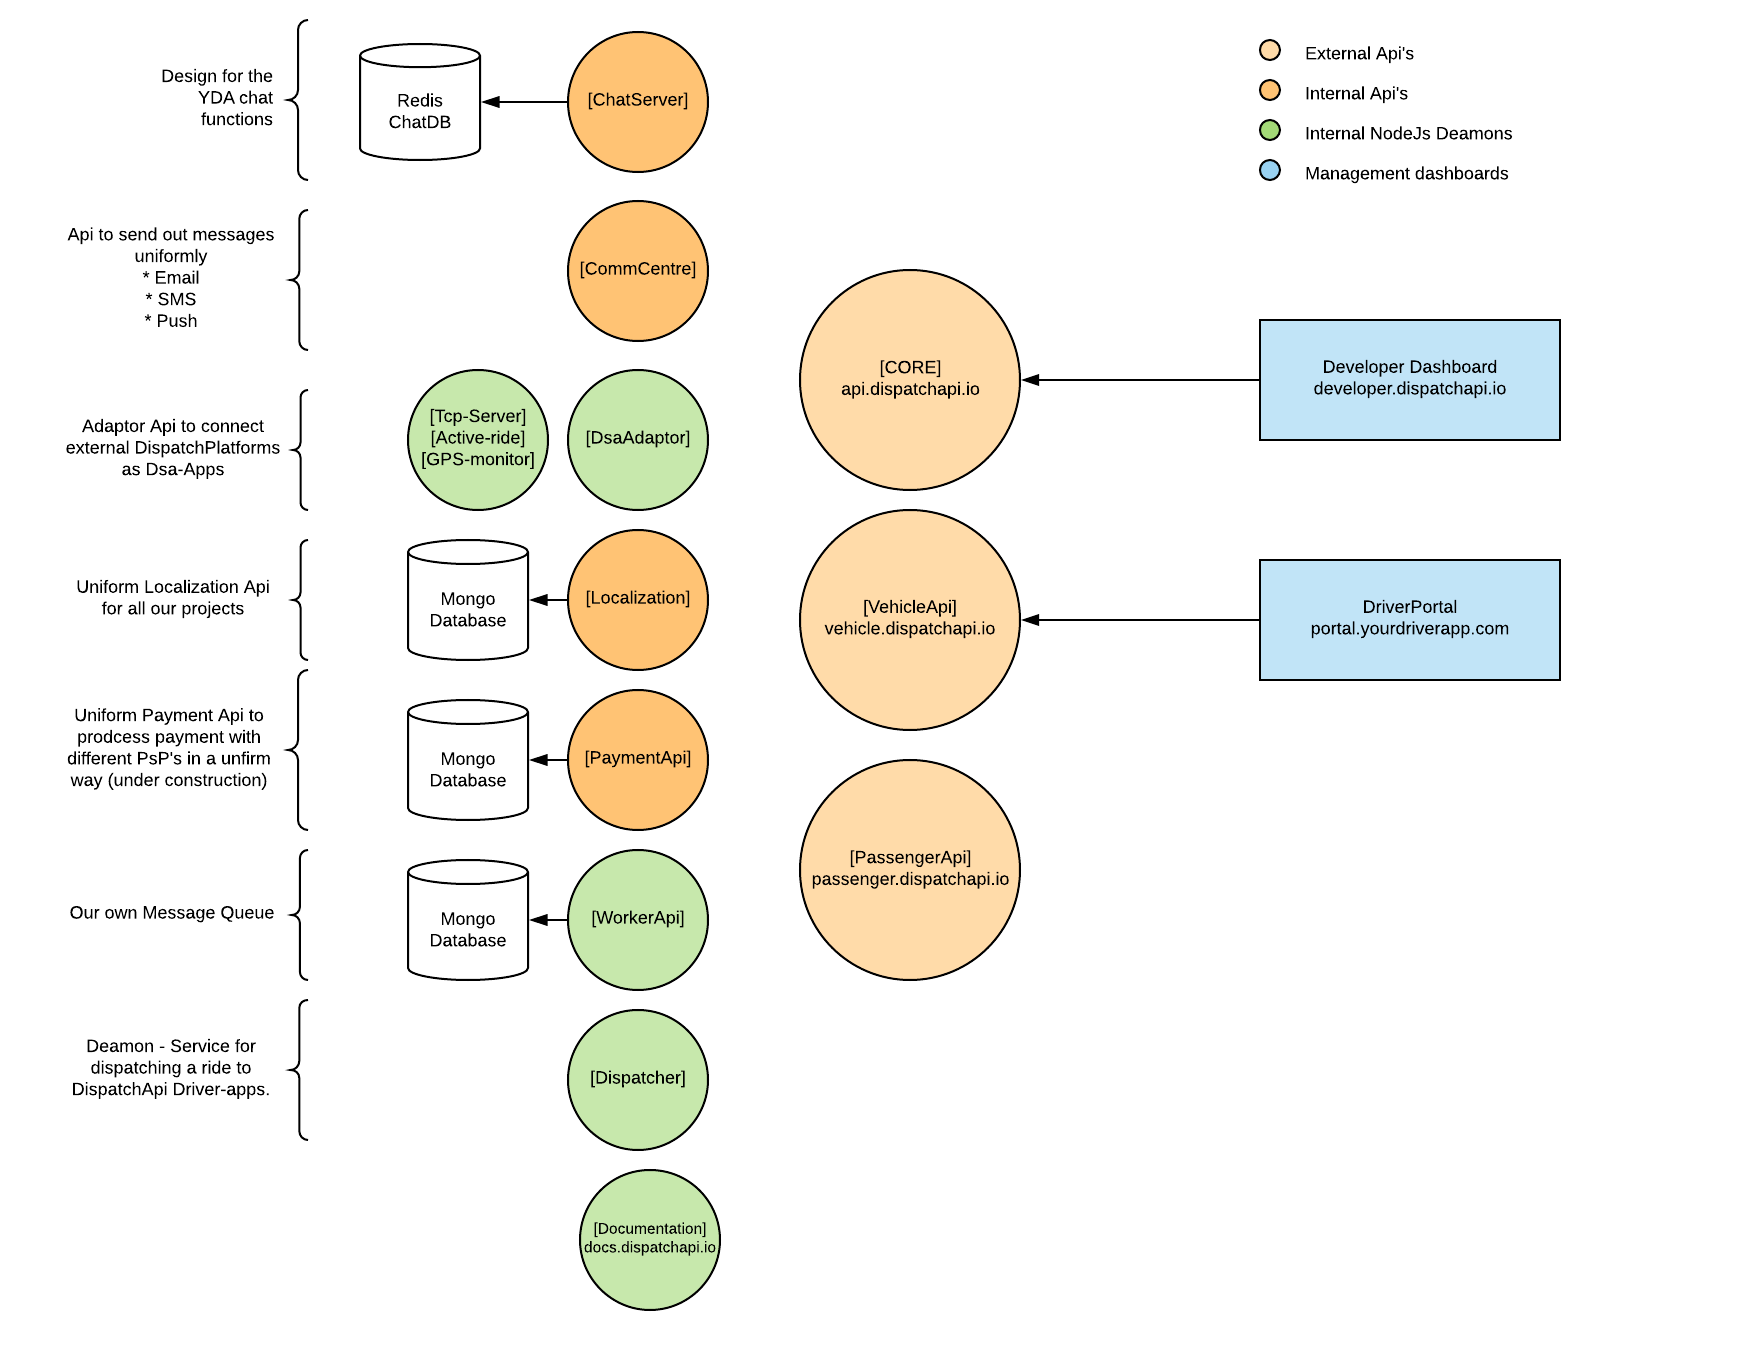
\includegraphics[width=1\textwidth]{Architecture}
	\caption[Architecture]{Current System Architecture provided by taxiID}
	\label{fig:Architecture}
\end{figure}

\subsection{Monoliths and Microservices}
Monoliths are large single upright blocks of stone, especially shaped into or serving as a pillar or monument. In the context of computer softare, a monolithic system may have different meanings. Rod Stephens captures the meaning of a monolithic architecture quite broadly: "In a monolithic architecture, a single program does everything. It displays the user interface, accesses data, processes customer offers, prints invoices, launches missiles, and does whatever else the application needs to do" in \cite{rod-BSE}.

\subsection{Functional Decomposition}

What logically follows from implementing functionalities as components in monoliths is either duplication or dependence between larger systems. This  contradicts an important principle of software engineering; don't repeat yourself (DRY), or limits scalability and indedpendence of deployment.

The legacy system has implemented its price calculation system in this manner, now facing difficulties of expanding the functionality to new projects. If the previous price calculation system was implemented as a microservice, it could have been reused or deployed as a second separate price calculation system for YDA. Fiar points of criticism have been made in regard to microservices. Jan Stenberg has pointed out that microservices are information barriers in \cite{JS-microservices}, meaning that the process of implementing a new system is degraded by the sense of ownership of specific services by developers. Technical downsides that have been discussed in general are: latency, testing, deployment, and message formats. As with most technological decisions, whether a microservice is desired depends on the problem that it meant to solve. When should a system be integrated or separated? It is a careful balancing between efficiency of satisfying dependencies keeping a separation of concern, and duplication of functionalities.

Integration of the backend would mean that the core system would contain the price calculation system as a component, separation of the backend would mean that the backend would be set up as a separate service. Integration of the frontend would mean that the DriverPortal would contain the views to manipulate information in the backend, separation of the frontend would mean that the views would be delivered from a separate service, or from within the backend service as a single project.

Building the TPS frontend and backend into one single project would be in conflict with this three-tier pattern, which would not be desired unless the decision is made to provide the frontend as iframes.

% \begin{itemize}
% 	\item Integrating frontend into existing portal, creating new service for backend
% 	\item Creating ser
% \end{itemize}

%%%%%%%%%%%%%%%%%%%%%%%%%%%%%%%%%%%%%%%%%%%%%%%%%%%%%%%%%%%%%%%%%%%%%%%%%%%%%%%%
% Accessing Necessary Data
%%%%%%%%%%%%%%%%%%%%%%%%%%%%%%%%%%%%%%%%%%%%%%%%%%%%%%%%%%%%%%%%%%%%%%%%%%%%%%%%
% - Which data are required to make TPS operational?
%
\section{Information Dependencies}
TPS will provide two types of services based around the same data. Portal users can mutate pricing information, mobile apps can retrieve trip prices. To effectively calculate the price of a ride, or to allow the portal user to mutate pricing data, the app or portal sending the request must be identified and authorized, which will be discussed in the next section. Assuming this has succesfully been achieved, some data may or may not be required from other services or databases in the system architecture. In the case of a price calculation, some extra required data are sent in the body of the request:

\begin{enumerate}
	\item vehicleTypes: string[]
	\item passengerCount: number
	\item requestedDate: ISODate
	\item departure: \{ gps: \{ lat: string, lng: string \} \}
	\item destination: \{ gps: \{ lat: string, lng: string \} \}
\end{enumerate}

In both the price calculation and the portal data mutation case, required data are stored in one or more databases. The proposed database schema for TPS in Image 4.7.1. of Appendix \ref{appendix:pregame} shows the general structure of the data that must be stored for TPS to be operational. A large portion of that data are only relevant for price calculations, and should therefore not be stored in existing databases. Data that are relevant to all systems may include but not be limited to:

\begin{enumerate}
	\item Company
	      \begin{enumerate}
		      \item name
		      \item Country
		      \item taxing / VAT
		      \item Application
	      \end{enumerate}
	\item Country
	      \begin{enumerate}
		      \item name
		      \item language
		      \item default VAT
	      \end{enumerate}
	\item Appliation
	      \begin{enumerate}
		      \item name
	      \end{enumerate}
\end{enumerate}

A decision must be made whether company and product information is stored


%%%%%%%%%%%%%%%%%%%%%%%%%%%%%%%%%%%%%%%%%%%%%%%%%%%%%%%%%%%%%%%%%%%%%%%%%%%%%%%%
% Authentication and Authorization
%%%%%%%%%%%%%%%%%%%%%%%%%%%%%%%%%%%%%%%%%%%%%%%%%%%%%%%%%%%%%%%%%%%%%%%%%%%%%%%%
% - How can authentication between services be implemented or improved?
%
\section{Authentication and Authorization}
% Current implementation


Each microservice is responsible for managing and containing state to enable users who would like to use the system to be authenticated and authorized. Advantages of a microservice are the fact that a microservice is a self-contained and has a naturally modular structure. But authentication and authorization must be handled by the microservice itself, unless state is shared amongst services. In the current system architecture, different services implement different authentication methods, store different pieces of information of different users. Authorization is managed by sending extra headers for each crucial piece of information, this is clarified in Appendix \ref{appendix:pregame}, chapter 3.4. For example: company information, application information, and user information is all sent in separate headers. When the amount of services that are added to the architecture increases, the mount of information that is no longer centralized increases with it. Mobile applications should be able to make requests, just like the portals that are to be developed. But portal users make use of the microservice in a different way. Mobile apps merely request prices of products, based on the rules that group admins define through the portal. To make sure that only the portal users have the right to mutate their data, users have to be authenticated and authorized within the microservice. Identity management becomes a problem if data duplication is not desired. If a user makes a direct request to the microservice, the credentials have to be compared to user data in a database. To prevent duplication, the microservice could be connected to the database that is used by the core system. But this makes the microservice less decoupled, and directly contradicts the desire to separate concerns. Four examples demonstrate this problem:

\begin{itemize}
	\item Example 1: The microservice authenticates and authorizes users all by itself, managing sessions and storing user data in its database.
	\item Example 2: The microservice connects to an exising databases to acquire the required information about the user.
	\item Example 3: The core system authenticates the user and provides a token that can be verified by the microservice, containing user identity.
	\item Example 4: A separate service is used for authentication and authorization so that the core system is not involved at all.
\end{itemize}

In the first example, the microservice seems to work independently, because it has knowledge about the users identity without making requests to adjacent systems, or connecting to external databases. But this is not true. If data about the user is mutated in the core system, the microservice needs to be notified or synced. This greatly hinders scaling and makes it harder to keep data consistent. Example two solves the inconsistency part by connecting to the central database that holds user data, but contradicts the strive for encapsulation.

\subsection{JSON Web Tokens}
Example three entirely removes the database connection to any user data. This is possible when a JSON Web Token (JWT) is used. A JWT may be signed with a cryptographic algorithm or even a public/private key pair using RSA. After the user enters valid credentials, the core system validates the credentials by comparing them with user data in the database. The core system signs a token that with a secret that is known by the microservice. The token consists of three parts, separated by a fullstop. The first part (header) of the token contains information about the hashing algorithm that was used to encrypt the payload. This part is Base64Url encoded. The payload itself contains information stored in JSON format:

\mynote{Show diagram with hierarchy of companies and apps}

\begin{center}
	\begin{tikzpicture}
		\draw  (-2,5) rectangle (1,3);
	\end{tikzpicture}
\end{center}

\begin{Verbatim}[fontsize=\scriptsize]
	{
		"companyId": "59ea0846f1fea03858e16311",
		"daAppInstallId": "599d39b67c4cae5f11475e93",
		"iat": 1521729818,
		"exp": 1521816218,
		"aud": "tps.dispatchapi.io",
		"iss": "api.dispatchapi.io",
		"sub": "getPrices"
	}
\end{Verbatim}

The identity of the user is stored in the payload that can only be revealed by whoever holds the secret with which it was signed. Then the message can be verified using the third part of the token, which is the signature. This verification step prevents tampering with the payload.

\subsection{oAuth 2.0}
Example four delegates managing user identity to a separate authentication service that, similar to the pricing microservice, has its own single task of authenticating users. OAuth 2.0 is a protocol that has been designed to allow third-party apps to grant access to an HTTP service on behalf of the resource owner. This behaviour could be utilized to allow users to make use of services within the architecture, controlled by a single service, stored in a single token. A proposal was made in the Pregame document to combine oAuth with JWT and an API Gateway to introduce an automated authentication flow with a single token, instead of sending multiple headers, see Appendix \ref{appendix:pregame}.

\begin{figure}[ht!]
	\centering
	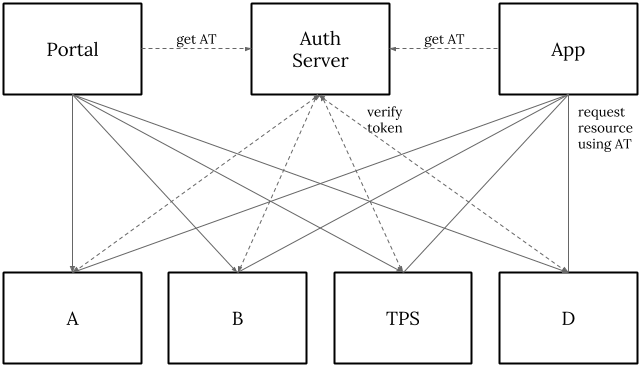
\includegraphics[width=.7\textwidth]{Auth1}
	\caption[Architecture]{OAuth requests where tokens are verified by Auth Server}
	\label{fig:Auth1}
\end{figure}
\clearpage
\begin{figure}[ht!]
	\centering
	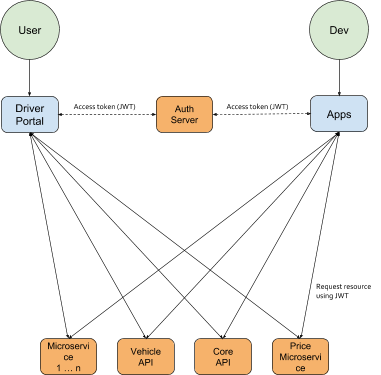
\includegraphics[width=.7\textwidth]{Auth2}
	\caption[Architecture]{OAuth with stateless JWT token requests}
	\label{fig:Auth2}
\end{figure}
\clearpage
\begin{figure}[ht!]
	\centering
	
\includegraphics[width=.7\textwidth]{Auth3}
	\caption[Architecture]{API Gateway}
	\label{fig:Auth3}
\end{figure}
\clearpage

\subsection{API Gateway}

Another common structure that allows services to be used by external agents is the API Gateway. It allows for a central middleware in which authentication and authorization is handled, where the microservices are shielded from public access, and all communication is established through the API Gateway [4].

Next to authentication, the gateway could optimize the endpoints so that no multiple requests are needed from external agents to gather different types of resources. These calls could be made internally to the microservices behind the gateway. This also opens the possibility the freely change the microservices without changing the public endpoints exposed by the gateway, and even offers slow or instant transitions to different versions of microservices.

The different proposals explain the improvements they may bring over some system. But the advice given is not tied to this project, instead to the entire Dispatch API. It’s advised to have a constructive dialogue about the future of the company, and the way it’s planning to scale. One could put a API Gateway in front of a monolithic app to help with transitioning to a microservice-oriented app.

%%%%%%%%%%%%%%%%%%%%%%%%%%%%%%%%%%%%%%%%%%%%%%%%%%%%%%%%%%%%%%%%%%%%%%%%%%%%%%%%
% Authentication and Authorization
%%%%%%%%%%%%%%%%%%%%%%%%%%%%%%%%%%%%%%%%%%%%%%%%%%%%%%%%%%%%%%%%%%%%%%%%%%%%%%%%
% - Which methods and technologies can be used to ensure suitability and
%   improve maintainability and testability?
%
\section{Suitability of Methods and Technologies}
\mynote{Write chapter about methods and technologies}
\begin{itemize}
	\item Node JS, PHP, MongoDB, MySQL, Microservice, Loopback, Graph QL,
	\item Slides and proposals
	\item Mocha, Buddy-Works, Circle CI, Typescript, Chai, Functional Programming
\end{itemize}
